\documentclass[paper=letter, fontsize=14pt]{scrartcl} 


\usepackage[utf8]{inputenc}
\usepackage{color}
\usepackage{hyperref}
\usepackage{graphicx}
\usepackage{epsfig}
\usepackage{multirow}
\usepackage{colortbl}
\usepackage[table]{xcolor}
\usepackage{fancyhdr}
\usepackage{graphicx}
\usepackage{graphicx}
\usepackage{verbatim}
\usepackage{pictex}  
\usepackage{multimedia}
\usepackage{listings}
\usepackage{vmargin}
\usepackage{xcolor,colortbl}
\usepackage[spanish]{babel} % language/hyphenation
\usepackage{amsmath,amsfonts,amsthm} % Math packages
\usepackage{amsbsy}
\usepackage{amssymb}
\usepackage{fancyvrb}
\usepackage{sectsty} % Allows customizing section commands
\allsectionsfont{\centering \normalfont\scshape} % Make all sections centered, the default font and small caps

\usepackage{fancyhdr} % Custom headers and footers
\pagestyle{fancyplain} % Makes all pages in the document conform to the custom headers and footers
\fancyhead{} % No page header - if you want one, create it in the same way as the footers below
\fancyfoot[L]{} % Empty left footer
\fancyfoot[C]{} % Empty center footer
\fancyfoot[R]{\thepage} % Page numbering for right footer
\renewcommand{\headrulewidth}{0pt} % Remove header underlines
\renewcommand{\footrulewidth}{0pt} % Remove footer underlines
\setlength{\headheight}{13.6pt} % Customize the height of the header

\numberwithin{equation}{section} % Number equations within sections (i.e. 1.1, 1.2, 2.1, 2.2 instead of 1, 2, 3, 4)
\numberwithin{figure}{section} % Number figures within sections (i.e. 1.1, 1.2, 2.1, 2.2 instead of 1, 2, 3, 4)
\numberwithin{table}{section} % Number tables within sections (i.e. 1.1, 1.2, 2.1, 2.2 instead of 1, 2, 3, 4)
\setpapersize{A4}
\setmargins{2.5cm}       % margen izquierdo
{2.4cm}                        % margen superior
{16.5cm}                      % anchura del texto
{23.42cm}                    % altura del texto
{10pt}                           % altura de los encabezados
{1cm}                           % espacio entre el texto y los encabezados
{0pt}                             % altura del pie de página
{2cm}                           % espacio entre el texto y el pie de página

\setlength\parindent{0pt} % Removes all indentation from paragraphs - comment this line for an assignment with lots of text

\newcommand{\horrule}[1]{\rule{\linewidth}{#1}} % Create horizontal rule command with 1 argument of height

\title{	
\normalfont \normalsize 
\textsc{Centro de Investigaci\'on en Matem\'aticas (CIMAT). Unidad Monterrey} 
\\ [25pt] 
\horrule{0.5pt} \\[0.4cm] % Thin top horizontal rule
\huge \textbf{Aplicación a portafolios}\\ 
\horrule{2pt} \\[0.5cm] % Thick bottom horizontal rule
}

\author{Ricardo Cruz} % Your name

\date{\normalsize\today} % Today's date or a custom date


\rhead{\begin{picture}(0,0) \put(-56.7,-50){
\includegraphics[width=20mm]{cimat.png}} \end{picture}}
\renewcommand{\headrulewidth}{0.5pt}

\pagestyle{fancy}

\begin{document}
\lstdefinestyle{customc}{
  belowcaptionskip=1\baselineskip,
  basicstyle=\footnotesize, 
  frame=lrtb,
  breaklines=true,
  %frame=L,
  %xleftmargin=\parindent,
  language=C,
  showstringspaces=false,
  basicstyle=\footnotesize\ttfamily,
  keywordstyle=\bfseries\color{green!40!black},
  commentstyle=\itshape\color{red!40!black},
  identifierstyle=\color{blue},
  stringstyle=\color{purple},
}

\lstset{breakatwhitespace=true,
  basicstyle=\footnotesize, 
  commentstyle=\color{green},
  keywordstyle=\color{blue},
  stringstyle=\color{purple},
  language=C++,
  columns=fullflexible,
  keepspaces=true,
  breaklines=true,
  tabsize=3, 
  showstringspaces=false,
  extendedchars=true}

\lstset{ %
  language=R,    
  basicstyle=\footnotesize, 
  numbers=left,             
  numberstyle=\tiny\color{gray}, 
  stepnumber=1,              
  numbersep=5pt,             
  backgroundcolor=\color{white},
  showspaces=false,             
  showstringspaces=false,       
  showtabs=false,               
  frame=single,                 
  rulecolor=\color{black},      
  tabsize=2,                  
  captionpos=b,               
  breaklines=true,            
  breakatwhitespace=false,    
  title=\lstname,             
  keywordstyle=\color{blue},  
  commentstyle=\color{dkgreen},
  stringstyle=\color{mauve},   
  escapeinside={\%*}{*)},      
  morekeywords={*,...}         
} 


\maketitle % Print the title


\pagebreak

\textbf{Ejercicio 1:}\\

Para el ejercicio 1 se buscará encontrar la frontera eficiente para un proceso en el cual se considera el 100\% de retorno esperado, $\Sigma=I$ y la matriz de covarianza muestral es modelada como un Ensemble de Wishart con $\sigma=.2$, además de considerar 100 activos durante 200 periodos.\\

Esto se implemento en el código \emph{ejercicio1.py}. El resultado se puede apreciar en la figura 1, donde se muestra el riesgo verdadero, así como el riesgo dentro y fuera de muestra. Se observa que a medida que la ganancia crece, los valores in y out se alejan del riesgo verdadero.

\begin{figure}[h]
\centering
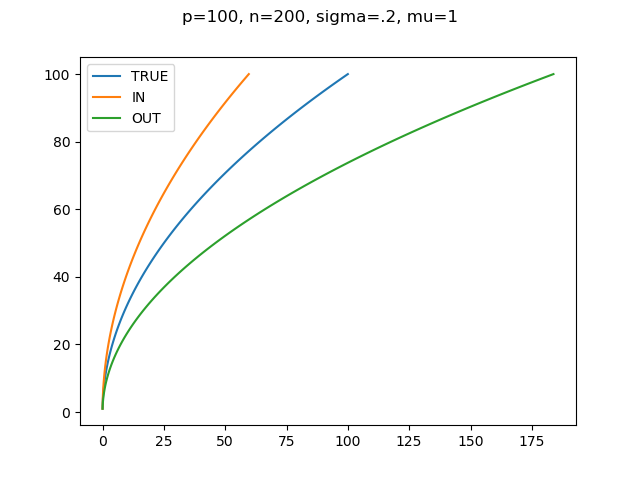
\includegraphics[scale=.75]{i1.png}
\caption{Riesgo verdadero, in y out} 
\end{figure}
\pagebreak

Además, se realizaron algunas pruebas, modificando los parámetros, a saber, el número de activos, los periodos, el retorno esperado y el retorno esperado.\\

La figura 2 muestra algunos casos donde se modificaron los parámetros mencionados anteriormente, solo se modificaba uno a la vez y los demás permanecian coomo fueron planteados inicialmente.

\begin{figure}[h]
\centering
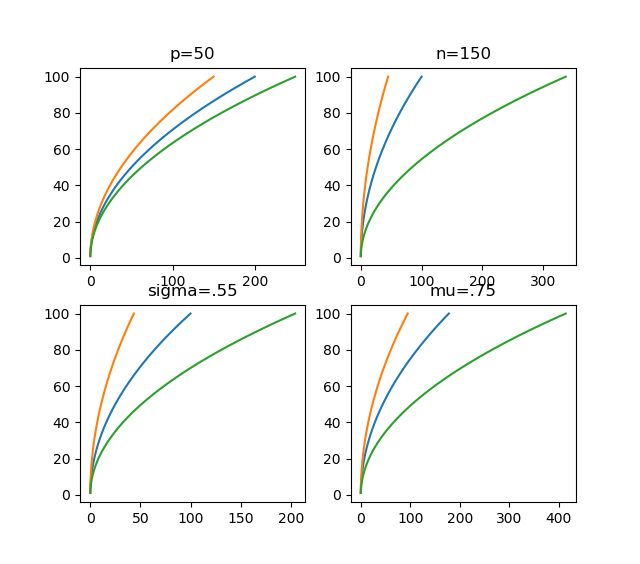
\includegraphics[scale=.75]{i2.png}
\caption{Sensibilidad a los parámetros.} 
\end{figure}

Se observa en las gráficas superiores, el valor de $p$ y $n$ influyen en que tan cercanos esta el riesgo in y out del verdadero, en general, si el valor de $n$ es grande respecto a $p$ se espera una gran cercanía.\\

En los gráficos inferiores, se aprecia que $\sigma$ y los retornos esperados influyen en la magnitud del riesgo, o su localización 

\pagebreak



\textbf{Ejercicio 2:}\\

El segundo ejercicio muestra como se puede limpiar la matriz de correlaciones, para que está modele el fenómeno de interes, descartando el ruido que tiene de manera implícita.\\

Para esto, en el código \emph{ejercicio2.py} se obtienen los rendimientos de 40 activos financieros de S\& P 500, considerando 218 periodos.\\

De manera general, la distribución de los valores propios puede ser acotada en valores que se ven superados por los verdaderos valores propios de la matriz de correlación muestral.\\

Por lo tanto, la matriz de correlaciones se replantea modificando la descomposición espectral de la matriz de correlaciones original, y asignando un valor fijo a los valores propios que sean menores a la cota o a un $i-esimo$ valor propio seleccionado.\\

La figura 3 muestra como existen valores propios mucho más grandes respecto a los valores propios más probables.

\begin{figure}[h]
\centering
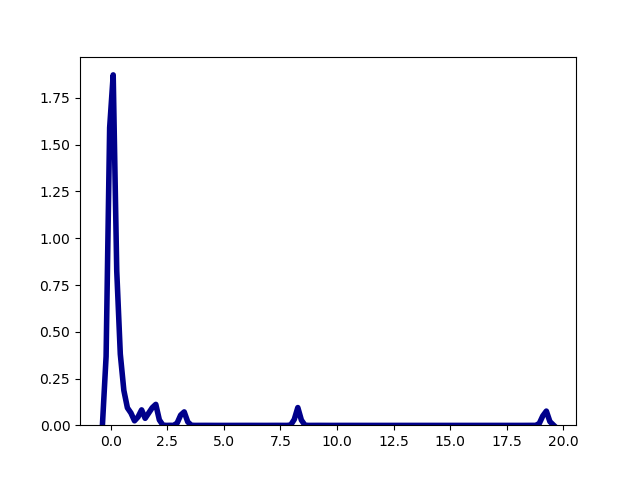
\includegraphics[scale=.75]{i3.png}
\caption{Distribución de los valores propios} 
\end{figure}
\pagebreak

Realizando esta corrección, los nuevos riesgo in y out son mas cercanos entre ellos. La figura 4 ilustra este comportamiento

\begin{figure}[h]
\centering
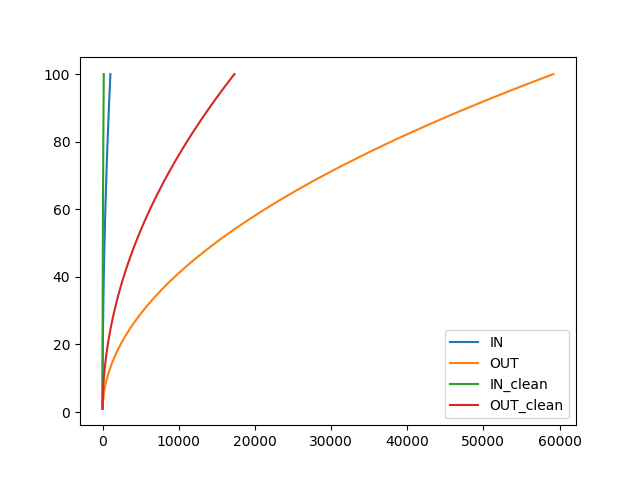
\includegraphics[scale=.75]{i4.png}
\caption{Riesgo in y out limpio} 
\end{figure}
\pagebreak


\end{document}
